\documentclass[pdf,9pt,aspectratio=169]{beamer}
\usepackage[utf8]{inputenc}

\AtBeginSection[]{
  \begin{frame}
  \vfill
  \centering
  \begin{beamercolorbox}[sep=8pt,center,shadow=true,rounded=true]{title}
    \usebeamerfont{title}\secname\par%
  \end{beamercolorbox}
  \vfill
  \end{frame}
}

\usepackage{DejaVuSans}
\usepackage{DejaVuSerif}
\usepackage{DejaVuSansMono}
\usepackage[T2A]{fontenc}

\usepackage[russian]{babel}

\usepackage{hyperref}
\hypersetup{unicode=true}

\usetheme{Madrid}
\usefonttheme[stillsansserifsmall]{serif}
%\usefonttheme[onlylarge]{structurebold}
\usefonttheme[onlylarge]{structureitalicserif}

\title[]{Архитектура компьютера}
\subtitle{Введение в предмет}
\author[]{Александр Рудалёв}
\institute[]{ИМИКТ САФУ}
\date[]{2016}

\usepackage{wrapfig}
\usepackage{color}
\usepackage{xcolor}

\usepackage{tikz}
\usetikzlibrary{arrows.meta}
\usetikzlibrary{babel}
\usetikzlibrary{shapes}
\usetikzlibrary{positioning}

\tikzset{
  MyChar/.style={
    rectangle, rounded corners=1mm,
    minimum height=6mm,
    minimum width=4.8mm,
    very thick, draw=black!50,
    top color=white,bottom color=black!20,
  },
}

\usepackage{minted}
\usemintedstyle{default} 
\newcommand{\cpil}[1]{\mintinline{python3}{#1}}

\begin{document}

\frame{\titlepage}

%%%%%%%%%%%%%%%%%%%%%%%%%%%%%%%%%%%%%%%%%%%%%%%%%%%%%%%%%%%%%%%%%%%%%%%%%%%%%%%
%%
%% Определения
%%
\begin{frame}\frametitle{Введение в предмет <<Архитектура компьютера>>}
  \begin{block}<1->{Определение}
    \textbf{Архитектура компьютера} "---  это описание его организации и принципов функционирования его структурных элементов. Включает основные устройства ЭВМ и структуру связей между ними.
  \end{block}
  \begin{block}<2->{О чём пойдёт речь}
    В рамках дисциплины мы должны понять как работает компьютер и программное обеспечение на нём.
  \end{block}
\end{frame}

%%%%%%%%%%%%%%%%%%%%%%%%%%%%%%%%%%%%%%%%%%%%%%%%%%%%%%%%%%%%%%%%%%%%%%%%%%%%%%%
%%
%% Содержание дисциплины
%%
\begin{frame}\frametitle{Содержание дисциплины}
  \begin{block}<1->{}
    \begin{itemize}
      \item Основы архитектуры ЭВМ (базовые части и их связи).
      \item Язык программирования Ассемблер (язык процессора).
      \item Компиляция, загрузка и выполнение программы.
      \item Инструменты программиста.
    \end{itemize}
  \end{block}
\end{frame}

%%%%%%%%%%%%%%%%%%%%%%%%%%%%%%%%%%%%%%%%%%%%%%%%%%%%%%%%%%%%%%%%%%%%%%%%%%%%%%%
%%
%% Введение в архитектуру ЭВМ
%%
\section{Введение в архитектуру ЭВМ}

%%%%%%%%%%%%%%%%%%%%%%%%%%%%%%%%%%%%%%%%%%%%%%%%%%%%%%%%%%%%%%%%%%%%%%%%%%%%%%%
%%
%% Вопрос
%%
\begin{frame}{Вопрос}
  \begin{columns}[c]
\only<1>{
    \begin{column}[]{0.5\textwidth}  
}
\only<2>{
    \begin{column}[]{0.35\textwidth}  
}
      \begin{alertblock}<1->{Что это?}
        \begin{figure}
          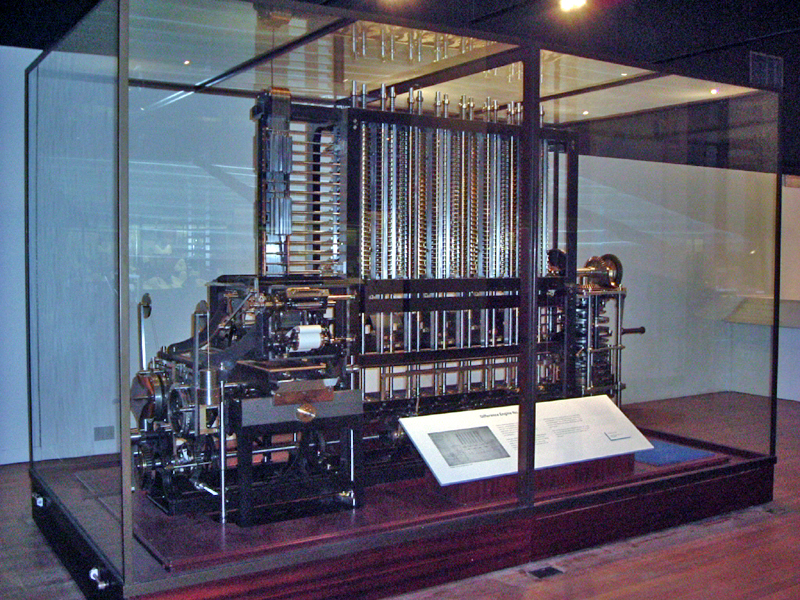
\includegraphics[width=\textwidth]{images/DifferenceEngine.jpg}
        \end{figure}
      \end{alertblock}
    \end{column}
\only<2>{
    \begin{column}[]{0.55\textwidth}
      \begin{exampleblock}<1->{Разностная машина Чарльза Бэббиджа}
        \begin{columns}[]
          \column{2cm}
            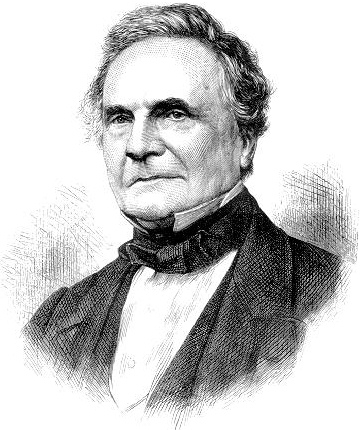
\includegraphics[width=\textwidth]{images/CharlesBabbage.jpg}
          \column{5.7cm}
              \setlength{\leftmargini}{5pt}
            \begin{itemize}
              \item До: Суммирующая машина Паскаля (1642 г.).
              \item Применение: Вычисление логарифмических таблиц.
              \item Первая статья: 1822 г.
              \item Реализация работающей копии: 1989-1991 гг.
            \end{itemize}
        \end{columns}
        \begin{itemize}
          \item Прообраз для: Аналитической машины.
          \item На её основе в 1854 г. Георг Шутц строит более простую <<машину вычислений>>.
          \item Р.С.~Гутер, Ю.Л.~Полунов <<От абака до компьютера>>
        \end{itemize}
      \end{exampleblock}
    \end{column}
}
  \end{columns}
\end{frame}

%%%%%%%%%%%%%%%%%%%%%%%%%%%%%%%%%%%%%%%%%%%%%%%%%%%%%%%%%%%%%%%%%%%%%%%%%%%%%%%
%%
%% Аналитическая машина Чарльза Бэббиджа
%%
\begin{frame}{Аналитическая машина Чарльза Бэббиджа}
  \begin{columns}[T]
    \begin{column}[]{0.45\textwidth}  
      \begin{exampleblock}<1->{Реализация}
        \begin{center}
          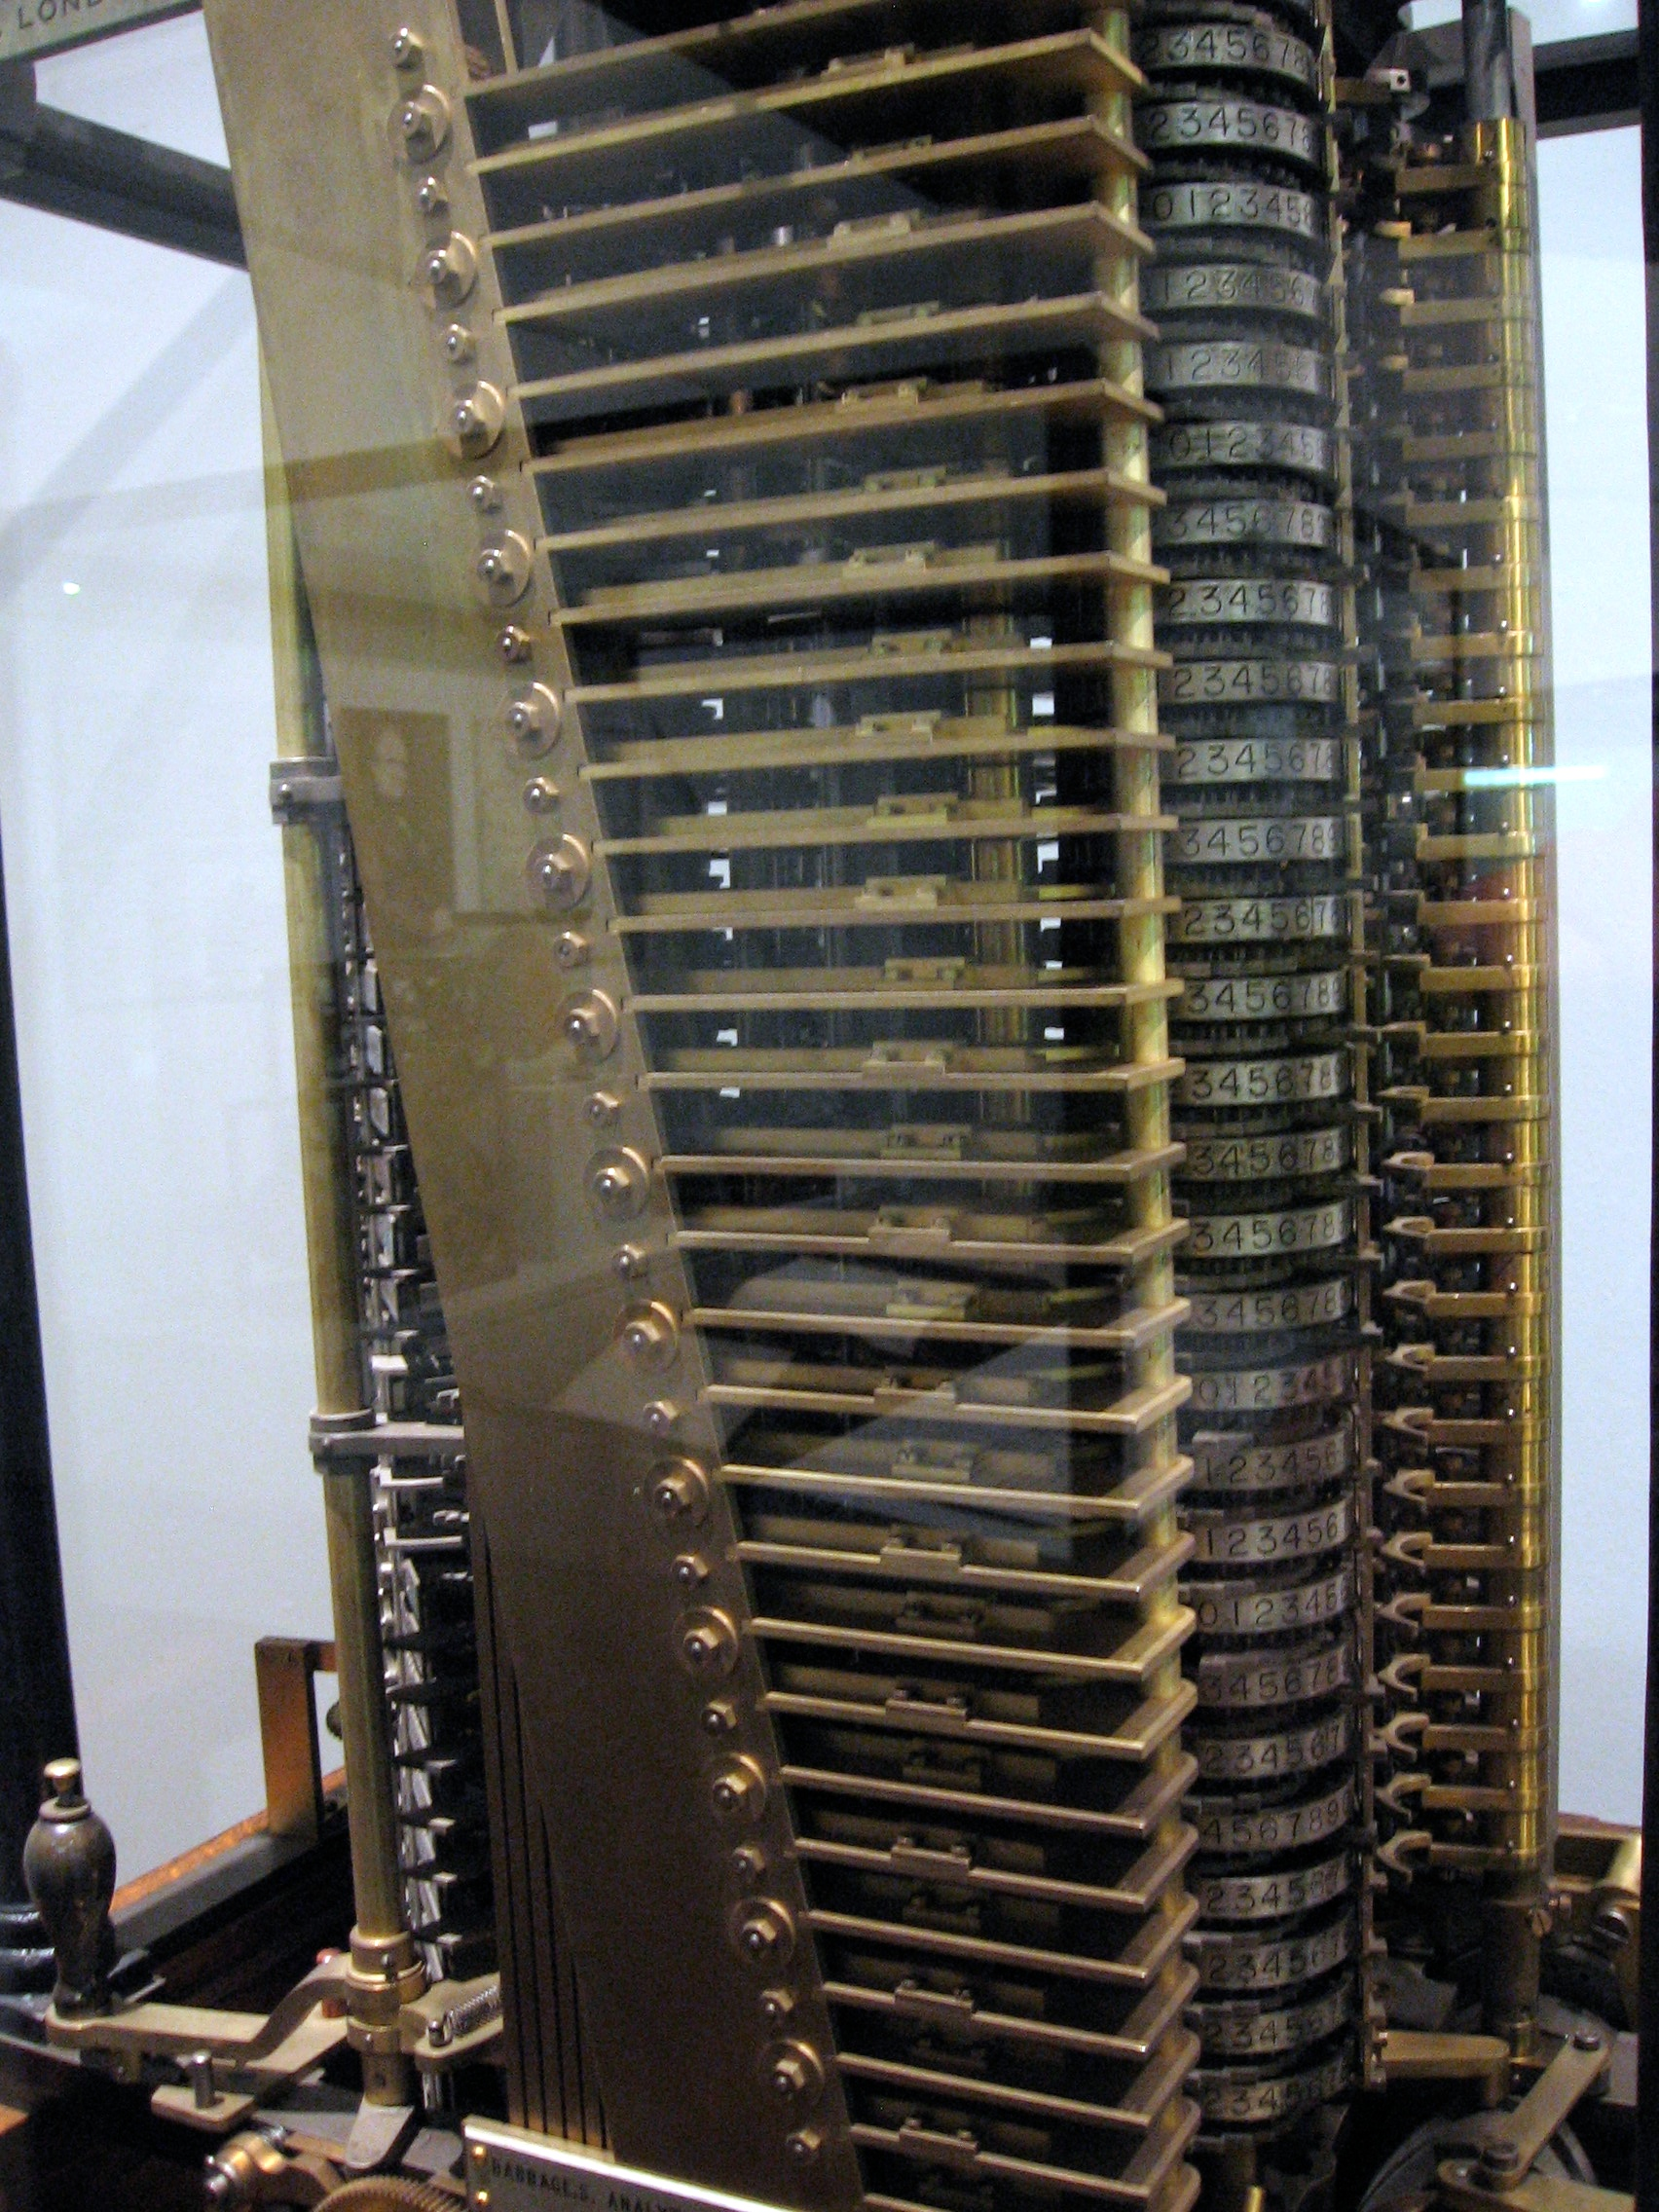
\includegraphics[height=.33\textheight]{images/AnalyticalEngineMill.jpg}\ 
          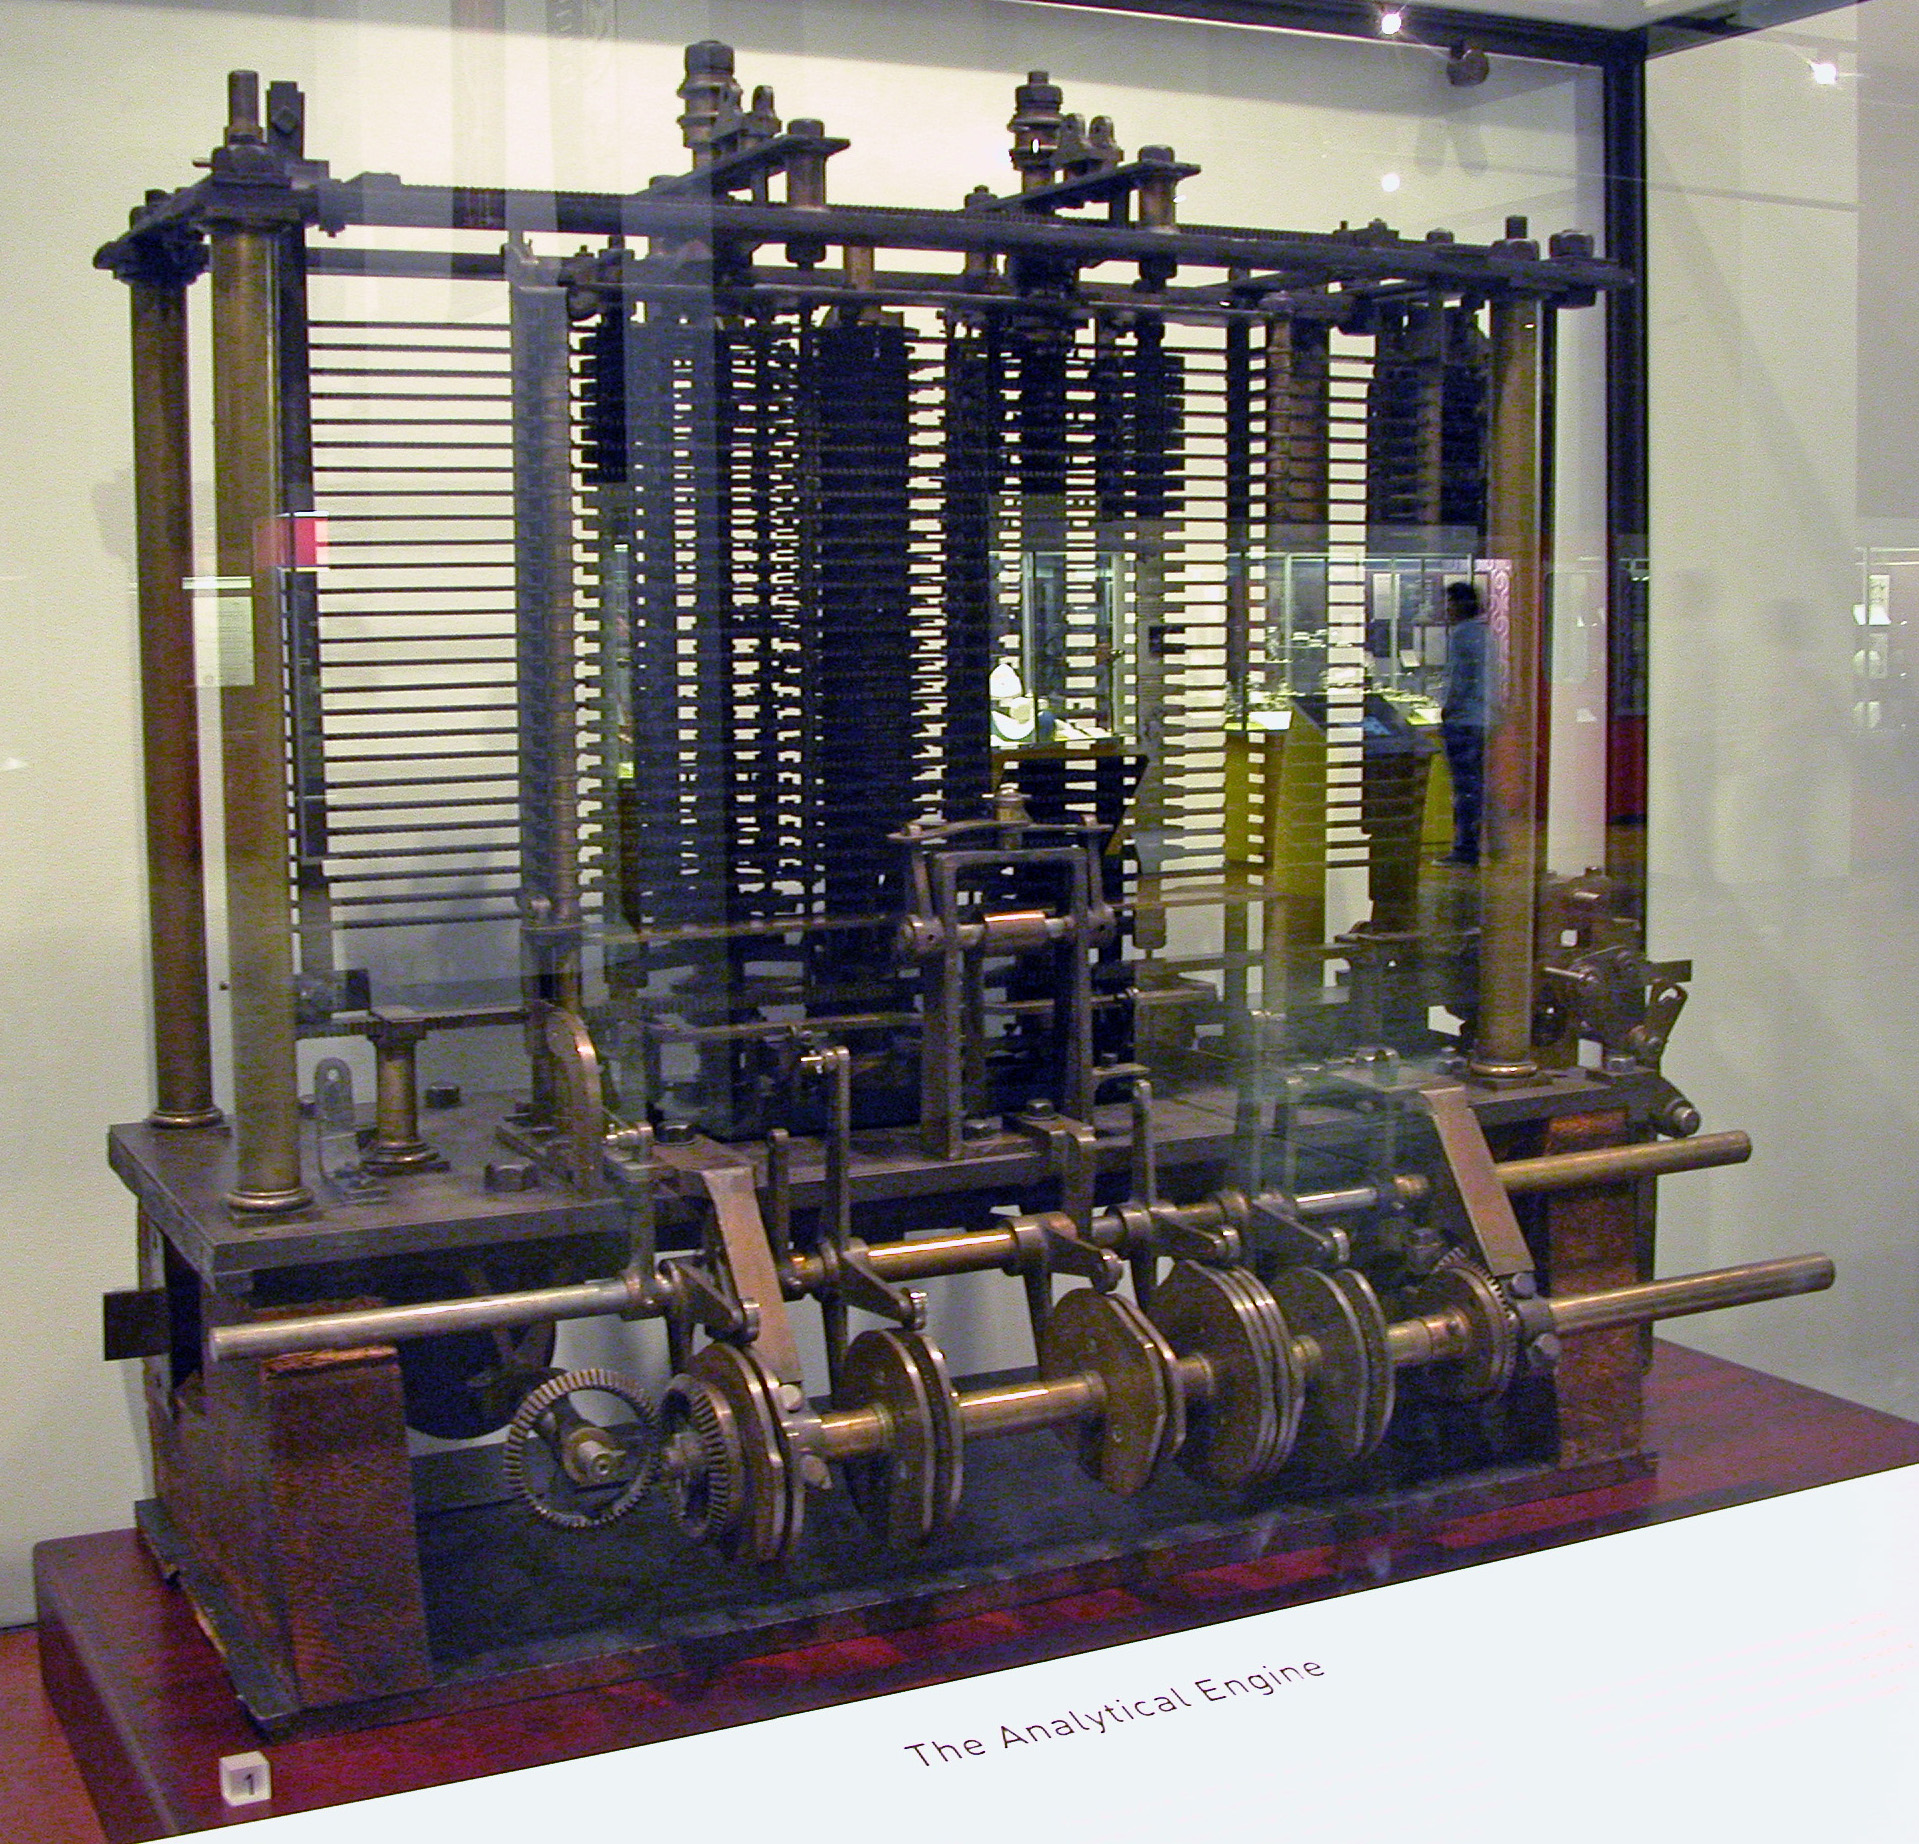
\includegraphics[height=.33\textheight]{images/AnalyticalEngineModel.jpg}\ 
          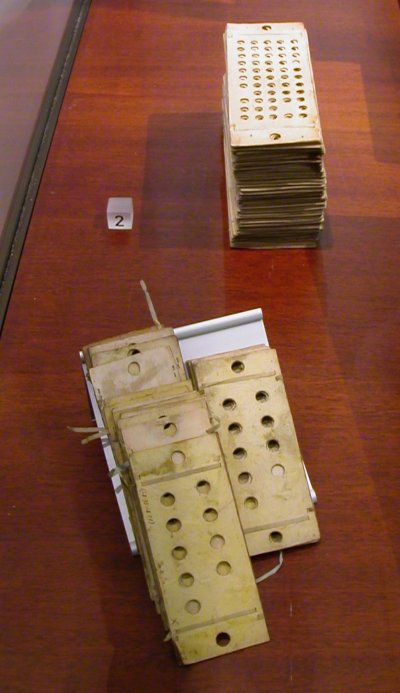
\includegraphics[height=.33\textheight]{images/AnalyticalEnginePunchedCards.jpg}
        \end{center}
      \end{exampleblock}
      \begin{block}{Состав}
        \begin{itemize}
          \item {<<Склад>>}.
          \item {<<Мельница>>}.
          \item Устройство управления.
          \item Устройства ввода и вывода данных.
        \end{itemize}
      \end{block}
    \end{column}
    \begin{column}[]{0.45\textwidth}  
      \begin{block}<1->{Интересные факты}
        \begin{itemize}
          \item {<<Склад>>} в 1000 чисел по 50 десятичных знаков.
          \item Система предварительного (сквозного) переноса при сложении.
          \item Ввод команд для мельницы и склада через  свои перфокарты (отдельные потоки для данных и команд).
          \item Условный переход в обе стороны.
          \item Первая программа: ???
        \end{itemize}
      \end{block}
    \end{column}
  \end{columns}
\end{frame}

%%%%%%%%%%%%%%%%%%%%%%%%%%%%%%%%%%%%%%%%%%%%%%%%%%%%%%%%%%%%%%%%%%%%%%%%%%%%%%%
%%
%% Архитектура фон Нейман
%%
\begin{frame}{Архитектура фон Неймана}
  \begin{columns}[c]
    \begin{column}[]{0.45\textwidth}  
      \begin{exampleblock}<1->{Схема}
        \begin{center}
          \begin{tikzpicture}
\node[MyChar, minimum width=3cm, minimum height=1.5cm, text width=2.7cm, align=center] (ALU) at (0,0) {Арифметико-\\логическое\\устройство};
\node[MyChar, minimum width=3cm, minimum height=1.5cm, text width=2.7	cm, align=center] (UU) at (-3.5cm,0) {Управляющее\\устройство};
\node[MyChar, minimum width=6.5cm] (MEM) at (-1.75cm,1.7cm) {Запоминающее устройство};
\node[MyChar, minimum width=6.5cm] (INOUT) at (-1.75cm,-1.7cm) {Устройства ввода/вывода};
\draw[<->,very thick, draw=black!50] (UU) to (ALU);
\draw[<->,very thick, draw=black!50] (UU) to (UU |- MEM.south);
\draw[<->,very thick, draw=black!50] (ALU) to (ALU |- MEM.south);
\draw[<->,very thick, draw=black!50] (ALU) to (ALU |- INOUT.north);
          \end{tikzpicture}
        \end{center}
      \end{exampleblock}
    \end{column}
    \begin{column}[]{0.45\textwidth}  
      \begin{block}<2->{Принципы}
        \begin{itemize}
          \item Однородности памяти.
          \item Адресности.
          \item Программного управления.
          \item Двоичного кодирования.
        \end{itemize}
      \end{block}
      \begin{exampleblock}<3->{EDSAC, Кембриджский университет, 1949 г.}
        \begin{center}
          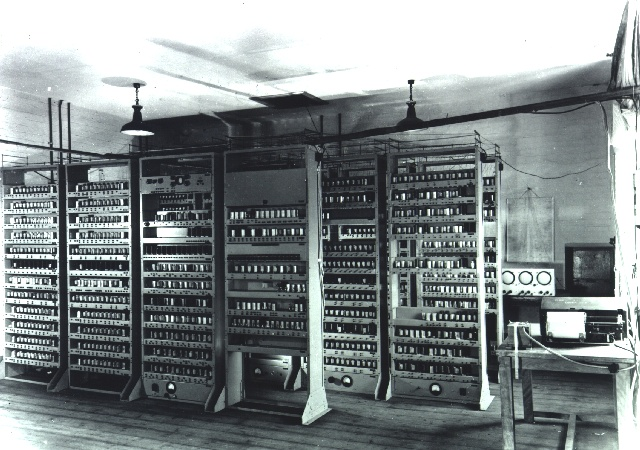
\includegraphics[height=.33\textheight]{images/EDSAC.jpg}
        \end{center}
      \end{exampleblock}
    \end{column}
  \end{columns}
\end{frame}

%%%%%%%%%%%%%%%%%%%%%%%%%%%%%%%%%%%%%%%%%%%%%%%%%%%%%%%%%%%%%%%%%%%%%%%%%%%%%%%
%%
%% Узкое место архитектуры фон Неймана
%%
\begin{frame}{Узкое место архитектуры фон Неймана}
  \begin{columns}[c]
    \begin{column}[]{0.45\textwidth}  
      \begin{exampleblock}<1->{Обращение к памяти}
        \begin{center}
          \begin{tikzpicture}
\node[MyChar, minimum width=3cm, minimum height=1.5cm, text width=2.7cm, align=center] (ALU) at (0,0) {Арифметико-\\логическое\\устройство};
\node[MyChar, minimum width=3cm, minimum height=1.5cm, text width=2.7	cm, align=center] (UU) at (-3.5cm,0) {Управляющее\\устройство};
\node[MyChar, minimum width=6.5cm] (MEM) at (-1.75cm,2.65cm) {Запоминающее устройство};
\node[MyChar, top color=red!20!white,bottom color=red!40!white, minimum width=1cm] (BUS) at (-1.75cm,1.55cm) {};
\node[MyChar, minimum width=6.5cm] (INOUT) at (-1.75cm,-1.7cm) {Устройства ввода/вывода};
\draw[<->,very thick, draw=black!50] (UU) to (ALU);
\draw[<->,very thick, draw=black!50] (UU) to (BUS);
\draw[<->,very thick, draw=black!50] (ALU) to (BUS);
\draw[<->,very thick, draw=black!50] (MEM) to (BUS);
\draw[<->,very thick, draw=black!50] (ALU) to (ALU |- INOUT.north);
\coordinate[yshift=0.15cm] (PM) at (-1.75cm,1.55cm);
\coordinate[yshift=-0.15cm, xshift=-0.15cm] (PU) at (-1.75cm,1.55cm);
\coordinate[yshift=-0.15cm, xshift=0.15cm] (PA) at (-1.75cm,1.55cm);
\fill[black!50] (PM) circle[radius=2pt];
\fill[black!50] (PU) circle[radius=2pt];
\fill[black!50] (PA) circle[radius=2pt];
\draw[very thick, draw=black!50] (PM) to (PU);

          \end{tikzpicture}
        \end{center}
      \end{exampleblock}
    \end{column}
    \begin{column}[]{0.45\textwidth}  
      \begin{alertblock}<1->{Проблема}
        Совместное использование шины для памяти программ и памяти данных.
      \end{alertblock}
    \end{column}
  \end{columns}
\end{frame}

%%%%%%%%%%%%%%%%%%%%%%%%%%%%%%%%%%%%%%%%%%%%%%%%%%%%%%%%%%%%%%%%%%%%%%%%%%%%%%%
%%
%% Гарвардская архитектура
%%
\begin{frame}{Гарвардская архитектура	}
  \begin{columns}[c]
    \begin{column}[]{0.45\textwidth}  
      \begin{exampleblock}<1->{Схема}
        \begin{center}
          \begin{tikzpicture}
\node[MyChar, minimum width=6.7cm, minimum height=1.7cm] (CPU) at (-1.75,0) {};
\node[MyChar, minimum width=3cm, minimum height=1.5cm, text width=2.7cm, align=center] (ALU) at (0,0) {Арифметико-\\логическое\\устройство};
\node[MyChar, minimum width=3cm, minimum height=1.5cm, text width=2.7	cm, align=center] (UU) at (-3.5cm,0) {Управляющее\\устройство};
\node[MyChar, minimum width=3.25cm] (MEMP) at (-3.375cm,1.7cm) {ЗУ программ};
\node[MyChar, minimum width=3.25cm] (MEMD) at (-0.125cm,1.7cm) {ЗУ данных};
\node[MyChar, minimum width=6.5cm] (INOUT) at (-1.75cm,-1.7cm) {Устройства ввода/вывода};
\draw[<->,very thick, draw=black!50] (ALU |- CPU.south) to (ALU |- INOUT.north);
\draw[<->,very thick, draw=black!50] (ALU |- CPU.north) to (ALU |- MEMD.south);
\draw[<->,very thick, draw=black!50] (UU |- CPU.north) to (UU |- MEMP.south);
          \end{tikzpicture}
        \end{center}
      \end{exampleblock}
    \end{column}
    \begin{column}[]{0.45\textwidth}  
      \begin{block}<1->{Основное отличие}
        \begin{itemize}
          \item Процессор может читать инструкции и выполнять доступ к памяти данных одновременно.
        \end{itemize}
      \end{block}
      \begin{exampleblock}<2->{Mark I, Гарвардский университет и IBM, 1944 г.}
        \begin{center}
          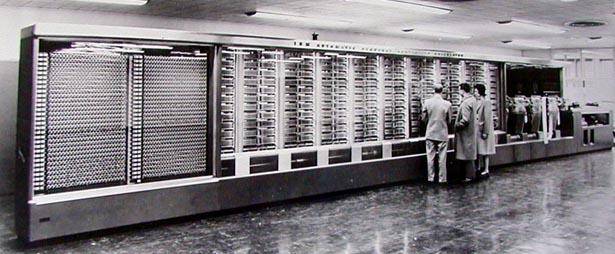
\includegraphics[height=.33\textheight]{images/HarvardMarkI.jpg}
        \end{center}
      \end{exampleblock}
    \end{column}
  \end{columns}
\end{frame}

%%%%%%%%%%%%%%%%%%%%%%%%%%%%%%%%%%%%%%%%%%%%%%%%%%%%%%%%%%%%%%%%%%%%%%%%%%%%%%%
%%
%% Инструменты
%%
\section{Инструменты}

%%%%%%%%%%%%%%%%%%%%%%%%%%%%%%%%%%%%%%%%%%%%%%%%%%%%%%%%%%%%%%%%%%%%%%%%%%%%%%%
%%
%% Инструменты
%%
\begin{frame}\frametitle{Инструменты}
  \begin{block}{Основные}
    \begin{itemize}
      \item<1-> Командная строка,
      \item<2-> NASM --- компилятор языка программирования Ассемблер,
      \item<3-> MinGW --- сборка компиляторов, библиотек и утилит на базе GCC для ОС Windows:
      \begin{itemize}
        \item GCC --- компилятор языка программирования Си,
        \item LD --- компоновщик,
        \item Make --- утилита для автоматизации процесса сборки программного обеспечения,
      \end{itemize}
      \item<4-> Mercurial --- система контроля версий.    
    \end{itemize}      
  \end{block}
  \begin{block}<5->{Дополнительные}
    \begin{itemize}
      \item Microsoft Visual Studio --- IDE, компиляторы, утилиты и библиотеки,
      \item CMake --- система автоматизации сборки программного обеспечения,
      \item ConEmu --- эмулятор терминала для ОС Windows.
    \end{itemize}      
  \end{block}
\end{frame}

%%%%%%%%%%%%%%%%%%%%%%%%%%%%%%%%%%%%%%%%%%%%%%%%%%%%%%%%%%%%%%%%%%%%%%%%%%%%%%%
%%
%% 
%%
\begin{frame}{}
  \begin{columns}[T]
    \begin{column}[]{0.45\textwidth}  
      \begin{exampleblock}<1->{}
        \begin{center}
        \end{center}
      \end{exampleblock}
    \end{column}
    \begin{column}[]{0.45\textwidth}  
      \begin{block}<1->{}
        \begin{itemize}
          \item
        \end{itemize}
      \end{block}
    \end{column}
  \end{columns}
\end{frame}

\end{document}
